\documentclass{ledger}
\usepackage{graphicx}
\usepackage{booktabs}
\usepackage{tabularx}
\usepackage{array}
\usepackage{amsmath,amssymb}
\usepackage{url}
\usepackage{xcolor}
\usepackage{listings}

\newcommand{\thefirstpagenum}[0]{X}
\newcommand{\thelastpagenum}[0]{X}
\newcommand{\theyear}[0]{2026}
\newcommand{\thevol}[0]{X}
\newcommand{\thedoi}[0]{DOI 10.5195/LEDGER.2026.XXXX}
\newcommand{\ledgerpages}[0]{\thefirstpagenum-\thelastpagenum}
\hypersetup{pdfauthor={Allemon, Adnan Omar Awad}, pdftitle={MOSAIC: State-Transition-Centric Integrity Capsules for Distributed Ledger Execution}}
\overfullrule=0pt

\title{MOSAIC: State-Transition-Centric Integrity Capsules for Distributed Ledger Execution}
\author{Adnan Omar Awad Allemon,\thanks{A. O. A. Allemon (adnanomar774@gmail.com) is an independent researcher.}}
\pagestyle{pagemain}
\pretitle{\centering \selectfont RESEARCH ARTICLE \par Submission Under Consideration at Ledger \par \fontsize{24pt}{28pt}\selectfont}

\begin{document}
\maketitle
\thispagestyle{pagefirst}

\begin{abstract}
Many distributed ledgers make a globally ordered block or log the primary unit of agreement, even when transactions touch disjoint state. This paper presents MOSAIC (Mutual-Obligation State And Integrity Capsules), a state-transition-centric protocol prototype in which a \emph{Capsule} names a predecessor state, carries an operation and witness obligations, and can be closed only by a quorum-backed \emph{ClosureProof}. A resulting \emph{StateSeal} authenticates the successor state. Conflicting claims are retained as signed evidence rather than silently discarded. The implementation combines a leaderless TCP dissemination layer, durable SQLite write-ahead logging, Ed25519 signatures, weighted membership and settlement, commit--reveal randomness, erasure-coded availability, deterministic execution, and a hash-chained event log. In a seven-process local rehearsal with two Byzantine test identities, a kill/restart event, and partial-frame denial-of-service probes, all 120 requested operations succeeded; the measured liveness ratio was 1.0, unexpected operational errors were zero, median latency was 37.52 ms, and p95 latency was 231.33 ms. These are local-emulation results, not Internet-WAN or public-testnet evidence. The contribution is therefore a reproducible protocol and systems artifact with a clearly bounded claim, rather than a claim of universal blockchain superiority.

\begin{keywords}
\item State-transition integrity.
\item Distributed-ledger protocol.
\item Byzantine fault tolerance.
\item Conflict evidence.
\item Deterministic execution.
\item Data availability.
\item Reproducible systems.
\end{keywords}
\end{abstract}

\section{Introduction}
Blockchains are often presented through the abstraction of a chain of blocks \cite{Nakamoto2008}, but the engineering problem that a ledger must solve is more specific: independent machines must agree on which state transitions are valid, how conflicting transitions are resolved, and how an observer can later verify the result. A total order is a useful general solution, yet it also forces unrelated activity through common ordering and commit paths. Modern systems have consequently explored other decompositions. HotStuff provides a responsive leader-based Byzantine fault-tolerant replication protocol with linear communication during key phases \cite{Yin2019HotStuff}; Narwhal separates reliable transaction dissemination from ordering and combines a causal DAG mempool with BFT consensus \cite{Danezis2022Narwhal}; FastPay uses Byzantine consistent broadcast rather than full consensus for a pre-funded settlement system \cite{Baudet2020FastPay}; and Sui Lutris combines a consensusless path with a high-throughput consensus path for transactions whose access patterns require ordering \cite{Blackshear2024SuiLutris}. These results show that the block is not the only possible unit around which integrity and agreement can be organized.

MOSAIC explores a different unit: the authenticated state transition. Its basic object, called a Capsule, commits to a resource, a predecessor StateSeal, an operation, a nonce, and the witness conditions under which another node may acknowledge the transition. A validator may issue a signed WitnessReceipt, but receipts do not by themselves mutate state. A first-claim lock prevents a validator from acknowledging two competing claims for the same resource in the same protocol context. Once a quorum of compatible receipts exists, a ClosureProof binds the accepted Capsule to the witness set and the predecessor. Deterministic execution then computes a successor state root, which is represented by a new StateSeal. If incompatible claims are observed, the protocol retains ConflictEvidence or an AbandonProof. This lifecycle is intended to make both positive and negative protocol events auditable.

The central research question is deliberately narrower than the phrase “a better blockchain”: can a state-transition-centric lifecycle provide a useful integrity boundary for distributed execution while preserving explicit evidence for conflicts and supporting crash recovery? The work does not assume that a different data structure automatically produces higher throughput, stronger security, or permissionless deployment. Those properties require formal assumptions, fair baselines, and independent network experiments. The present paper instead makes three contributions. First, it defines the MOSAIC object and closure lifecycle, including the relationship among predecessor seals, witness receipts, first-claim locks, closure proofs, execution roots, and conflict evidence. Second, it provides an executable Python prototype that integrates protocol, networking, storage, execution, availability, randomness, settlement, onboarding, and event logging rather than treating these as unrelated sketches. Third, it reports a reproducible local multi-process evaluation and clearly separates the measured results from claims that remain unverified.

The paper is organized as follows. Section 2 positions MOSAIC against adjacent ledger and BFT designs. Section 3 defines the protocol model and state-transition lifecycle. Section 4 describes the implementation. Section 5 presents the evaluation methodology and results. Section 6 discusses security assumptions, limitations, and the path to independent WAN evaluation. Section 7 concludes.

\section{Related Work and Positioning}

\subsection{Ordered replication and DAG-based dissemination}
HotStuff is a partially synchronous, leader-based BFT replication protocol. Its contribution is not merely a fast message path; it combines responsiveness with linear communication in the number of replicas and provides a framework relating several BFT protocols \cite{Yin2019HotStuff}. MOSAIC does not replace HotStuff's safety argument or claim a lower communication bound. Instead, it changes the object that an implementation exposes to its execution and audit layers. In a HotStuff-style ledger, a block or proposal is the natural carrier of ordered commands. In MOSAIC, the carrier is a Capsule whose validity is tied to a particular predecessor seal and resource scope. A future comparison must therefore use equivalent workloads and should not compare the local prototype's latency with a published HotStuff throughput number.

Narwhal and Tusk separate dissemination from ordering. Narwhal provides reliable dissemination and storage of causal histories, while Tusk supplies an asynchronous consensus protocol; their evaluation demonstrates the value of the separation under wide-area configurations and faults \cite{Danezis2022Narwhal}. MOSAIC shares the principle that availability and ordering should be explicit rather than hidden inside a monolithic block path. It differs in emphasis: its protocol object records an obligation-bearing transition and its negative outcomes are first-class evidence. MOSAIC's current availability layer is an erasure-coded local component, not a demonstrated replacement for a large-scale DAG mempool or a dedicated data-availability network.

\subsection{Local certificates and object-centric execution}
FastPay demonstrates that a high-integrity settlement system for pre-funded payments can use Byzantine consistent broadcast and avoid the expense of full atomic commit channels for its target workload \cite{Baudet2020FastPay}. Sui Lutris similarly combines consensusless agreement for suitable transactions with a consensus path for transactions at risk of inconsistent concurrent access; its paper also emphasizes the difficulty of safe reconfiguration \cite{Blackshear2024SuiLutris}. Sui's public documentation describes objects, versions, owners, and authenticated object references as the fundamental storage model \cite{SuiObjectModel}. MOSAIC is close to this family in its attempt to make independent state transitions explicit, but its object is not a smart-contract object and its current execution kernel is intentionally small. It supports deterministic SET, DELETE, and ADD\_INT-style instructions, nonce checks, gas accounting, and state roots; it does not provide a general-purpose virtual machine or a Move-like contract ecosystem.

Mysticeti shows that DAG-based BFT protocols can approach low message-round latency while maintaining a formal safety and liveness argument and a large-scale evaluation \cite{Babel2025Mysticeti}. This comparison is especially important for MOSAIC: a local p95 latency of 231.33 ms cannot be interpreted as evidence against systems evaluated on a WAN or as evidence of a new latency bound. The appropriate scientific question is whether MOSAIC's obligation and evidence lifecycle supplies a distinct correctness or accountability benefit at an acceptable cost under a common testbed.

\subsection{Position of the present contribution}
The novelty claim in this paper is a protocol composition claim, not a claim that gossip, quorum voting, Ed25519, Reed--Solomon coding, WAL recovery, or deterministic execution were individually invented here. MOSAIC proposes to use a Capsule--WitnessReceipt--ClosureProof--StateSeal lifecycle as the integrity boundary across execution, storage, availability, settlement, and event accountability. The combination may be useful, but its novelty relative to all prior work is not established by implementation alone. The paper therefore treats the design as a testable protocol hypothesis and provides artifacts so that independent researchers can challenge it.

\section{Protocol Model}

\subsection{Entities and state}
Let $R$ be a set of logical resources, such as an account, object, contract slot, or application-specific state domain. Each resource $r\in R$ has a current state root $s_r$. A StateSeal is a signed digest that identifies a network context, resource, predecessor seal, successor root, protocol epoch, and the validator or closure context that produced it. The implementation represents these values using canonical serialization and cryptographic digests.

A Capsule is modeled as
\begin{equation}
 C = (r, p, o, n, w, t, \sigma),
\end{equation}
where $r$ is the resource identifier, $p$ is the predecessor StateSeal identifier, $o$ is a deterministic operation, $n$ is a nonce, $w$ is the witness rule or required acknowledgement context, $t$ is a protocol timestamp or round context, and $\sigma$ is the originator's signature. A Capsule is not a state mutation. It is a signed claim that a transition may be attempted from $p$.

A WitnessReceipt is a signed statement by validator $v$ about a Capsule. The receipt records the Capsule digest, the validator identity, the decision, the relevant epoch, and any reason code. A receipt is valid only if its signature verifies, its referenced Capsule is canonical, and the validator has not already acknowledged an incompatible claim for the same resource and lock context.

\subsection{Mutual obligations and first claim}
The term mutual obligation describes the fact that a Capsule commits both the proposer and the potential witnesses to a common object. The proposer cannot later replace the predecessor, operation, or rule without producing a different Capsule digest. A witness cannot acknowledge an alternative Capsule for the same resource after acquiring a first-claim lock. The lock is local state, but its effect becomes globally relevant only through a closure quorum and the protocol's non-equivocation assumption.

For each resource $r$ and validator $v$, the protocol maintains a first-claim lock $L(r,v)$. Initially $L(r,v)=\bot$. A validator may transition the lock to $c$ only when it has verified $c$ and $L(r,v)=\bot$. The implementation rejects duplicate or replayed receipts and records protocol conflicts separately from unexpected operational errors. This distinction matters operationally: a Byzantine or stale message can be invalid without indicating that the daemon itself failed.

\subsection{Closure and successor seal}
Let $Q$ be a set of witnessing validators and let $\tau$ be the quorum threshold expressed either as a validator count in the local model or as a weighted stake threshold in the settlement-integrated model. A ClosureProof for Capsule $c$ and resource $r$ contains the predecessor identifier, Capsule digest, the compatible WitnessReceipts, the quorum context, and the closure identifier. Closure is accepted only if the receipts satisfy the quorum rule and the predecessor is known or is later resolved from durable state.

Deterministic execution applies the operation to the predecessor state. For the current kernel, the supported instruction family includes setting a key, deleting a key, and adding an integer value, with nonce and gas checks. If execution succeeds, the implementation computes a successor state root $s'_r$ and emits a StateSeal that commits to $c$, $s_r$, $s'_r$, and the ClosureProof. The state transition is persisted atomically with the relevant protocol event. A receipt whose predecessor root or successor root does not match the execution result is rejected.

\subsection{Conflict and abandonment evidence}
Suppose $c_1$ and $c_2$ reference the same resource and lock context but are incompatible. The protocol does not treat the losing claim as an unexplained absence. It creates ConflictEvidence containing the two claims and the verification context. If a claim cannot be closed because the necessary obligations are not satisfied, an AbandonProof may record the failure and its quorum or timeout context. These objects do not prove that every external observer agrees with the interpretation; they provide signed material that can be independently checked.

\begin{figure}
\centering
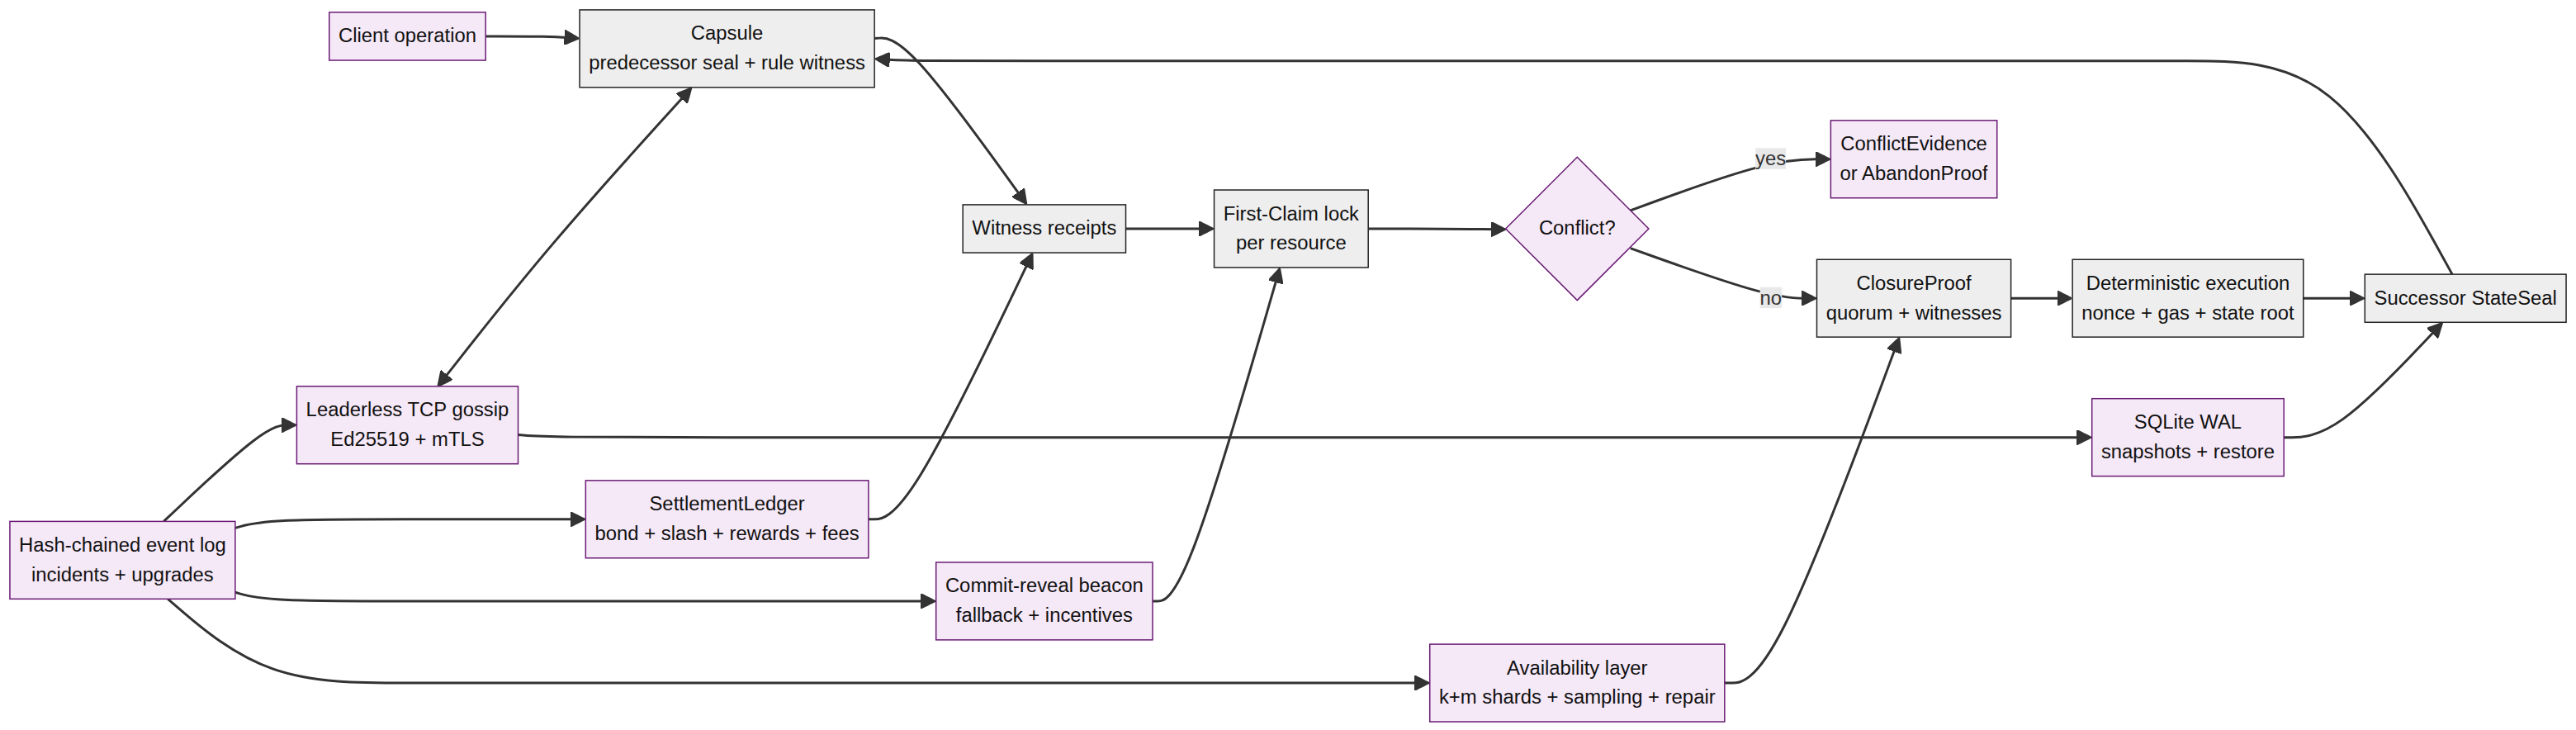
\includegraphics[width=1.0\textwidth]{figures/mosaic_architecture.png}
\caption{MOSAIC architecture. The Capsule--WitnessReceipt--First-Claim Lock--ClosureProof--execution--StateSeal path is the protocol core. Settlement, randomness, availability, networking, durable storage, and the event log are connected to this lifecycle rather than evaluated as independent services.}
\label{fig:architecture}
\end{figure}

\begin{figure}
\centering
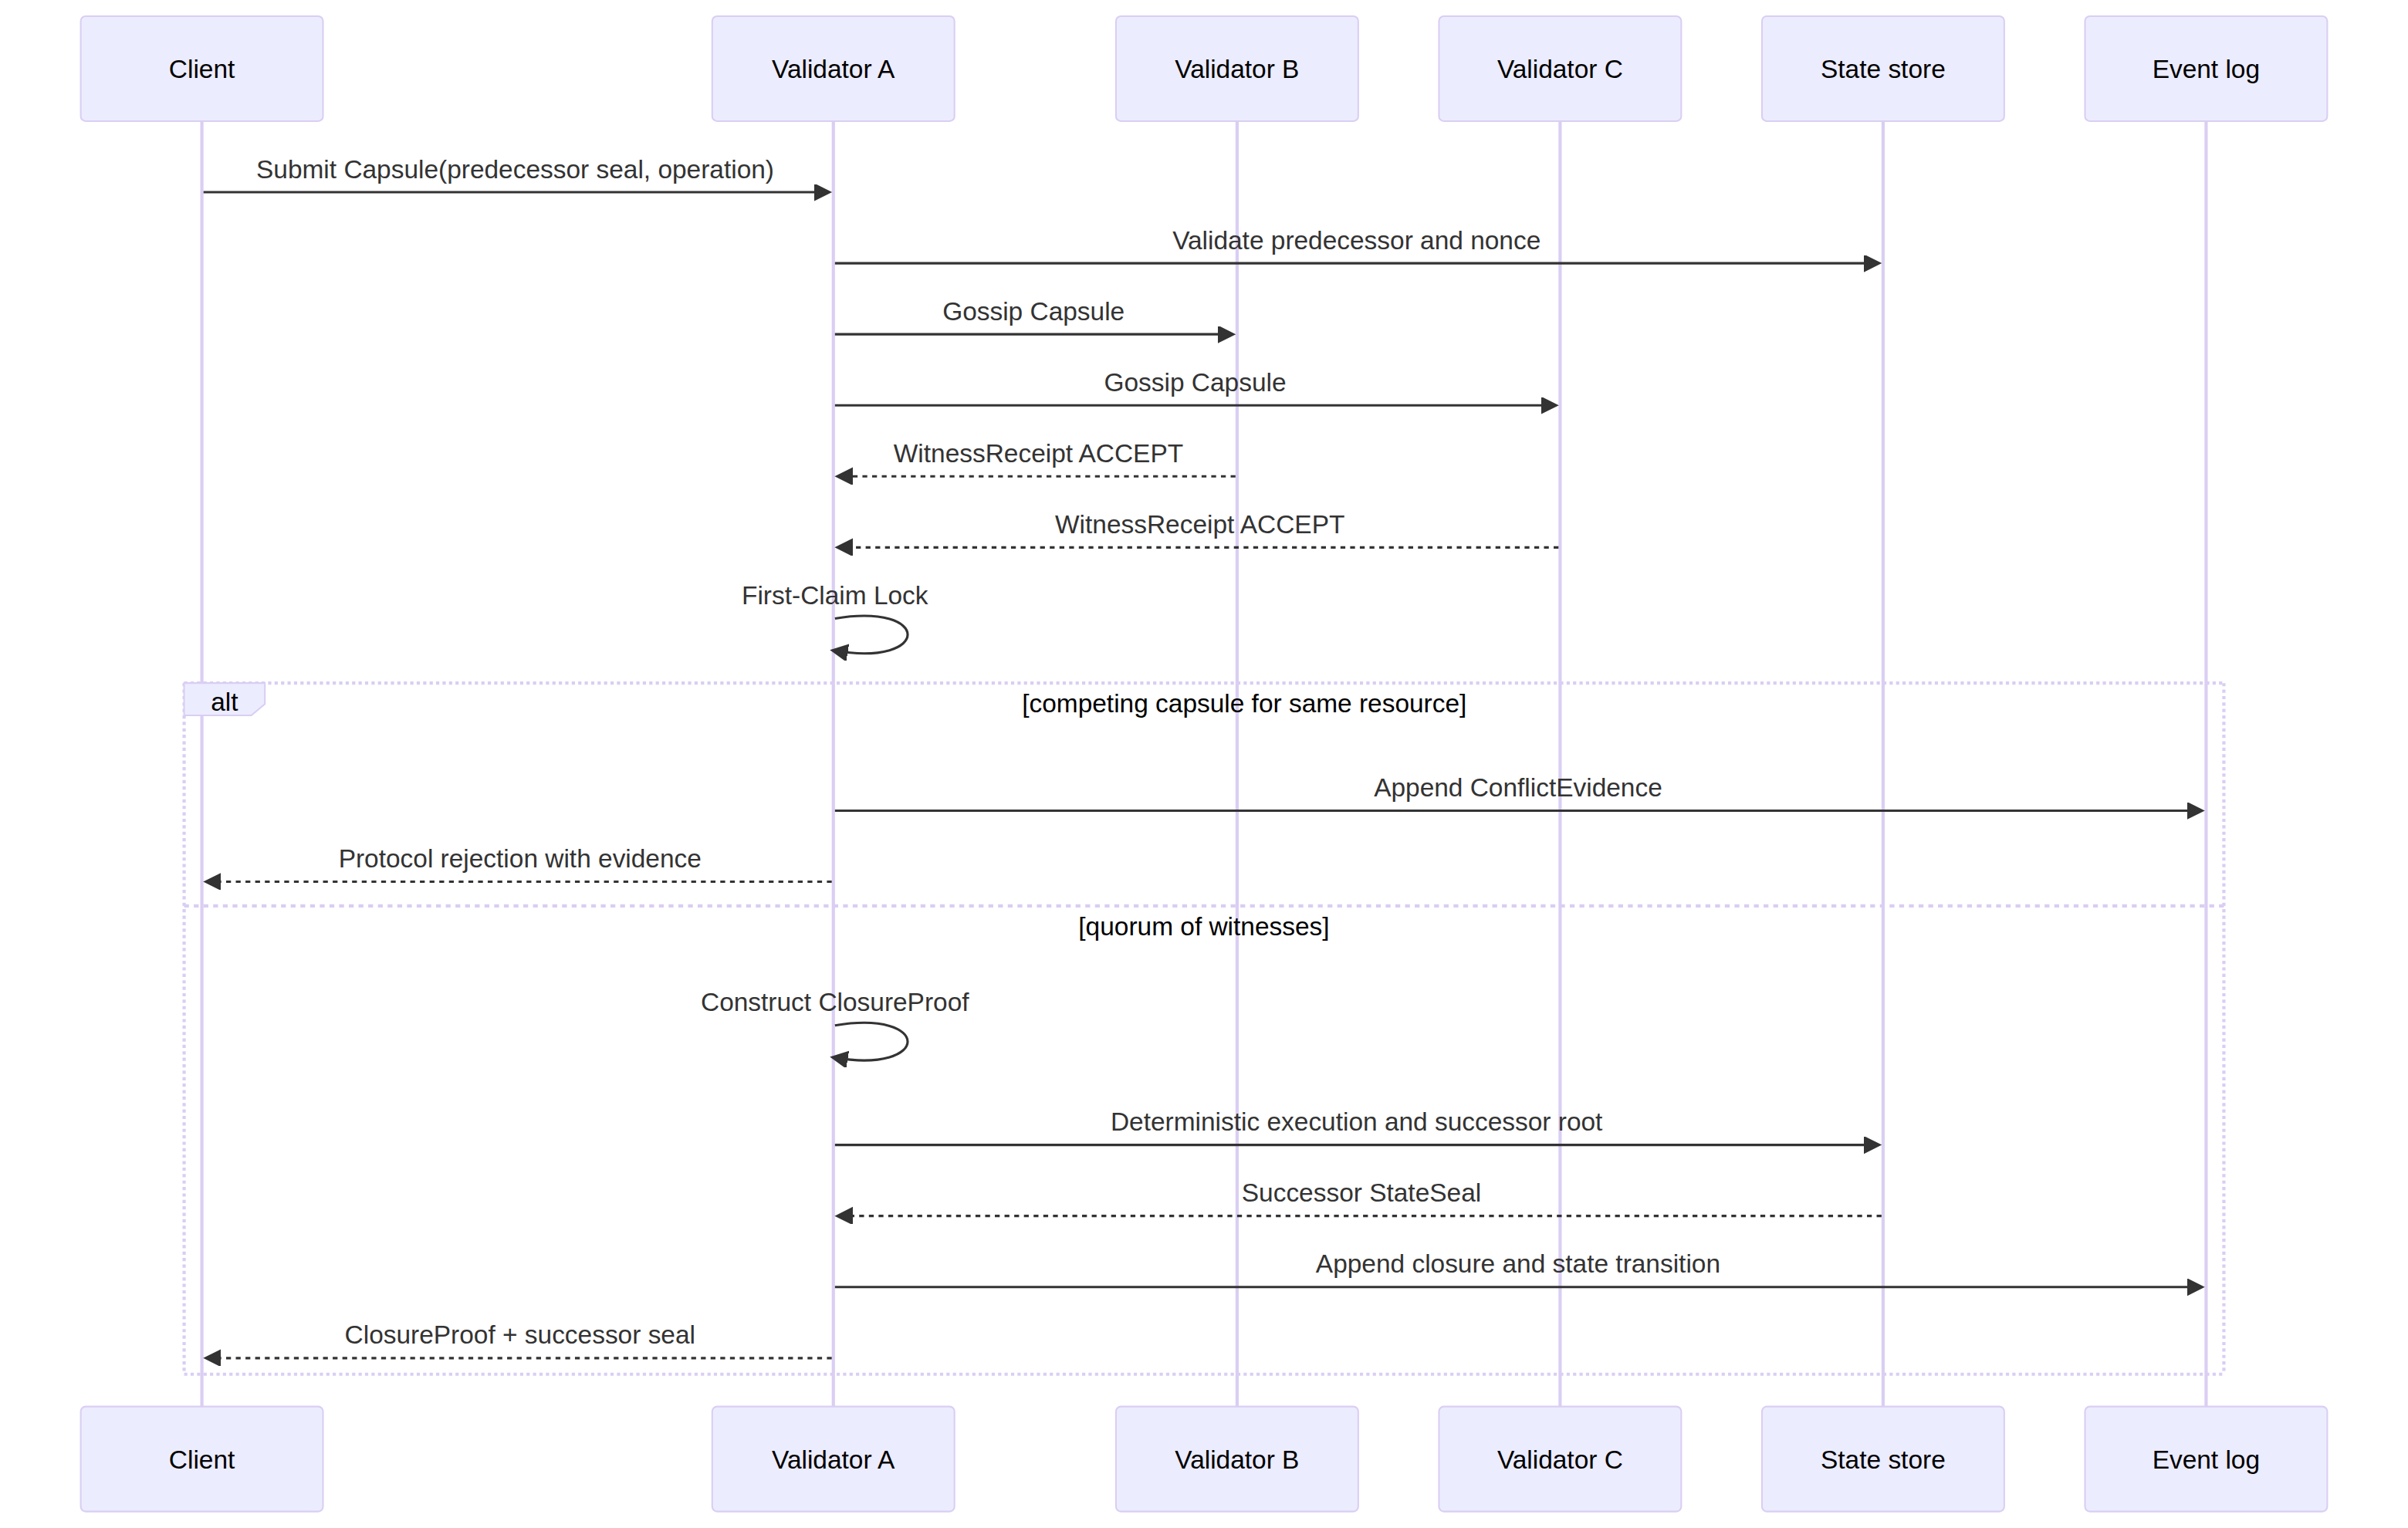
\includegraphics[width=0.94\textwidth]{figures/capsule_lifecycle.png}
\caption{A Capsule lifecycle with successful and conflicting paths. A validator first validates the predecessor and nonce, disseminates the Capsule, collects compatible receipts, and either appends conflict evidence or constructs a ClosureProof and successor StateSeal.}
\label{fig:lifecycle}
\end{figure}

\section{Implementation}

The prototype is written for Python 3.11 or newer. The package contains a \texttt{mosaic} namespace for the protocol and permissionless layers and a \texttt{ccd\_nexus} namespace for shared cryptographic primitives and legacy domain support. The public repository includes tests, benchmark harnesses, formal files, configuration examples, and the measured artifacts described in this paper.

\begin{table}[h]
\centering
\caption{MOSAIC protocol objects and their implementation roles.}
\label{tab:objects}
\begin{tabularx}{\textwidth}{p{3.2cm}X}
\toprule
Object & Role in the protocol \\
\midrule
StateSeal & Authenticated digest of a resource state and its transition context. \\
Capsule & Signed transition claim naming a predecessor, operation, nonce, and witness rule. \\
WitnessReceipt & Signed validator acknowledgement or rejection for a Capsule. \\
ClosureProof & Quorum-backed certificate that a Capsule may be applied. \\
ConflictEvidence & Evidence containing incompatible claims for the same resource context. \\
AbandonProof & Evidence that a claim was not closed under the applicable obligation or timeout context. \\
BundleClosure & Optional composition of several compatible closures. \\
\bottomrule
\end{tabularx}
\end{table}

\subsection{Networking and storage}
The network layer uses asyncio TCP connections with a four-byte length prefix and JSON payload framing. Messages are authenticated with Ed25519 signatures at the protocol layer. The node implementation supports optional mutual TLS, per-peer rate limits, replay protection, bounded frame sizes, frame timeouts, and connection caps. Gossip is leaderless in the sense that the dissemination layer does not require a single permanent coordinator to relay every Capsule.

Durability is provided by a SQLite WAL store with full synchronous mode, versioned schema support, snapshots, migration tests, and restore paths. The restart harness previously exposed a race in which a Capsule could be processed before predecessor seals had completed WAL restoration. The corrected path classifies an unknown predecessor as a retryable protocol rejection or pending item rather than an unexpected daemon error. This correction is included in the v5 results reported below.

\subsection{Membership, settlement, and randomness}
Membership is represented by signed admission requests, stake bonds, weighted committee selection, withdrawal delay, and slash evidence. SettlementLedger persists bonds, unbonding, rewards, penalties, and fees. The implementation is a local protocol component; it is not a legal or external token custody system and does not establish a public cryptocurrency economy.

The randomness layer uses commit--reveal rounds. A reveal that satisfies the round conditions contributes to the beacon; if the reveal quorum is not reached while a commitment condition remains sufficient, the implementation can use a commitment fallback. Non-reveal penalties and reveal rewards are recorded by the incentive manager. This is an operational mechanism, not a proof of incentive compatibility against all economic strategies.

\subsection{Availability and deterministic execution}
The availability layer uses Reed--Solomon coding over GF(256) with $k$ data shards and $m$ parity shards. It supports shard storage, sampling proofs, loss detection, and repair. The local availability network exposes PUT, FETCH, SAMPLE, and REPAIR message paths and persists artifacts through a WAL. The implementation is intended to make the data-availability assumption explicit; it has not been evaluated as a globally deployed availability network.

The execution kernel deliberately uses a small deterministic instruction set. A transaction contains an origin, nonce, gas limit, and ordered instructions. Execution verifies the predecessor root, applies the instructions atomically, checks gas and nonce rules, and returns a successor root and receipt. The kernel is suitable for studying protocol binding; it is not a general-purpose smart-contract virtual machine.

\section{Evaluation}

\subsection{Questions and scope}
The evaluation addresses four questions. First, does the implementation preserve its tested protocol invariants and reject malformed or replayed messages without unexpected exceptions? Second, can the integrated daemon complete a local multi-process workload under Byzantine test identities, a kill/restart event, and partial-frame probes? Third, did the restart-path correction remove the previously observed operational error and reduce the recovery tail? Fourth, are the resulting measurements sufficient to claim a public permissionless network or universal performance superiority? The answer to the fourth question is no, and that negative result is part of the evaluation.

The main experiment uses seven independent daemon processes on one host. Two identities, $w0$ and $w1$, are assigned Byzantine behavior by the harness; this is a deterministic test schedule, not an independent adversarial operator. The harness submits 120 operations, kills $w1$ at operation 40, restarts it from WAL, and opens 24 partial-frame connections to test bounded network handling. The measured scope is explicitly \texttt{LOCAL\_EMULATION}; it does not model Internet routing, independent hosts, clock skew across operators, NAT, heterogeneous bandwidth, or public participation.

\subsection{Verification gates}
The repository currently contains 87 automated tests covering protocol, membership, economics, storage, security, execution, onboarding, beacon, availability, and event-log behavior. A deterministic wire fuzz harness exercised 4,000 parser cases without an unexpected exception. The bounded model checker reports M1--M8 as passed. The model is intentionally bounded and abstracts cryptographic signatures through an honest non-equivocation assumption; it is not a complete formal proof.

\begin{table}[h]
\centering
\caption{Verification and rehearsal artifacts used in this paper.}
\label{tab:gates}
\begin{tabularx}{\textwidth}{p{4.1cm}p{2.0cm}X}
\toprule
Evidence & Result & Scope and interpretation \\
\midrule
Python test suite & 87/87 & Regression coverage for the repository's implemented paths. \\
Wire fuzz harness & 4,000 cases; 0 unexpected exceptions & Parser-level robustness; not a complete state-machine fuzzing proof. \\
Bounded model check & M1--M8 passed & Finite model with explicit abstractions; not an unbounded theorem. \\
Onboarding rehearsal & 4 daemons; gate passed & Local multi-process emulation. \\
Beacon rehearsal & 4 daemons & TCP commit, reveal, finalize, and settlement paths locally exercised. \\
Availability rehearsal & 5 daemons & Shard distribution, sampling, repair, and restart locally exercised. \\
Long-run rehearsal & 7 daemons; 120 operations & Byzantine schedule, kill/restart, partial-frame probes; one host. \\
Hash-chained event log & 8 events; verified & Append-only local record with chained event hashes. \\
\bottomrule
\end{tabularx}
\end{table}

\subsection{Long-run results}
The final v5 run completed all 120 requested operations. Its liveness ratio was 1.0, and the safety signal reported zero unexpected operational errors. Byzantine conflicts were retained as protocol evidence rather than counted as daemon failures. Median latency was 37.520503 ms and p95 latency was 231.326768 ms. The run sent 13,499,316 bytes and received 7,982,518 bytes, corresponding to approximately 179,015.28 bytes per successful operation under this workload and message schedule. The event log contained eight events and verified successfully. Twenty-four partial-frame connections were closed by the bounded network handler.

The preceding v3 run had exposed two \texttt{CapsuleInvalid: unknown predecessor seal} errors after restart and a p95 of 8,447.689336 ms. After the pending/rejection correction and recovery-path failover, v5 reported zero unexpected errors and a p95 of 231.326768 ms. Figure \ref{fig:latency} visualizes this change on a logarithmic y-axis. It is important not to interpret the improvement as a general protocol speedup: it is a correction to a recovery-path behavior in one local harness.

\begin{figure}
\centering
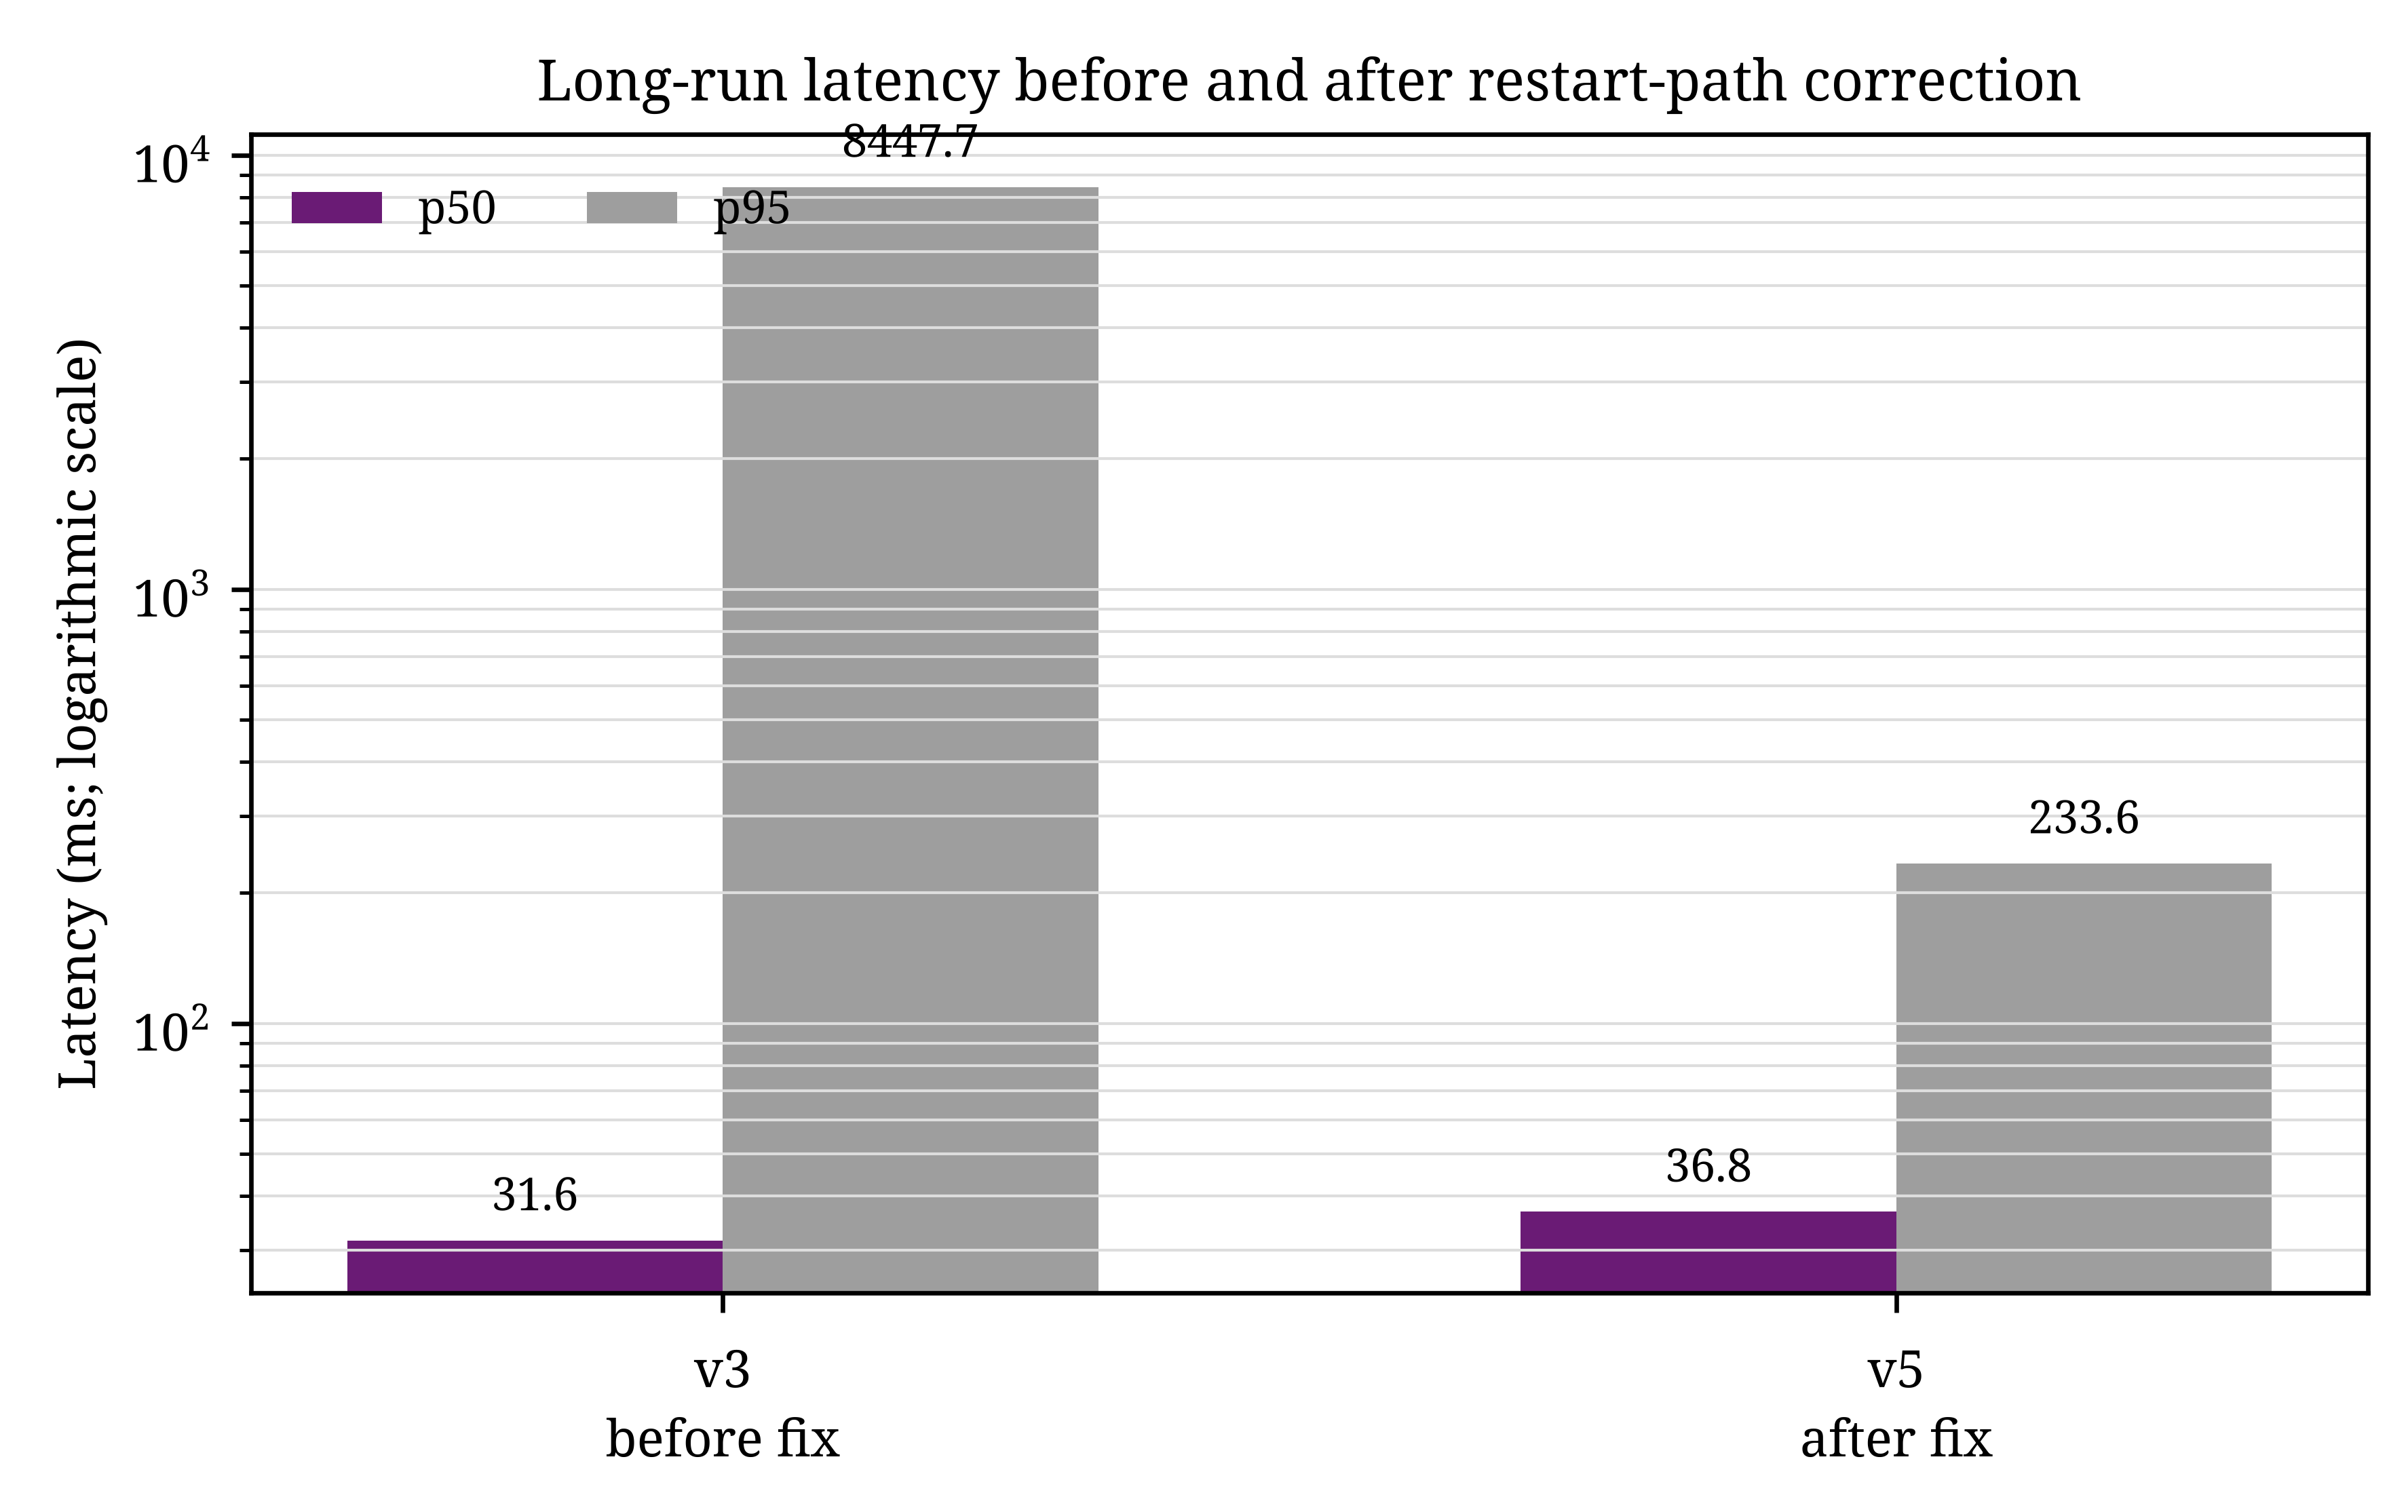
\includegraphics[width=0.93\textwidth]{figures/long_run_latency_comparison.png}
\caption{Measured p50 and p95 latency for the v3 and v5 local long-run artifacts. The logarithmic axis makes the former recovery tail visible. The v5 result follows the restart-path correction; both runs used the same seven-process local-emulation family and 120-operation workload.}
\label{fig:latency}
\end{figure}

\subsection{Interpretation of the measurements}
The measurements establish that the implementation can sustain the tested workload with complete operation success after a scheduled kill/restart and that the corrected path avoids classifying a recoverable predecessor race as an unexpected daemon error. They also show that the prototype has meaningful operational instrumentation: p50, p95, byte counters, protocol conflicts, replay rejections, rate limits, frame handling, and event-log verification are all exposed in the artifacts.

The measurements do not establish a throughput advantage over HotStuff, Narwhal/Tusk, Mysticeti, Sui Lutris, or any production ledger. The experiments are not conducted on the same hardware, network topology, client workload, payload size, execution semantics, storage engine, or fault schedule as the published baselines. In particular, published Narwhal/Tusk and Mysticeti evaluations report wide-area results that cannot be compared numerically with a localhost Python prototype \cite{Danezis2022Narwhal,Babel2025Mysticeti}. A fair comparison is a future experiment, not a conclusion of this paper.

\section{Security, Limitations, and Reproducibility}

\subsection{Security model}
The prototype assumes that signatures are unforgeable, canonical serialization is deterministic, honest validators do not equivocate within the modeled lock context, and a quorum threshold contains enough honest stake or validators for the intended BFT argument. It uses Ed25519 signatures and replay guards, but the paper does not claim resistance to compromised private keys, operating-system compromise, supply-chain attacks, or all denial-of-service strategies. The event log provides tamper-evident chaining within the log; it is not an external timestamp authority.

The first-claim lock is an integrity mechanism, not a full consensus proof. A safety theorem would need to define the quorum intersection under weighted stake, epoch changes, validator admission and removal, lock persistence, and the exact relation between local receipts and a globally accepted ClosureProof. The current TLA+ file is a bounded safety model. It records no-two-closures, no-apply-without-closure, conflict evidence, closure/abandon separation, availability quorum, and execution-receipt checks, but it intentionally abstracts cryptography and contains simplifications that must be replaced by nontrivial invariants before a formal claim is made.

\subsection{Permissionless and public-network limitations}
The settlement ledger is an executable accounting component, not an externally enforced economic system. A public network would additionally require token custody and issuance rules, a Sybil-resistant admission mechanism, stake concentration analysis, reliable slashing enforcement, operator key management, legal and governance policies, and independent economic review. The commit--reveal beacon improves liveness under non-reveal but does not alone prove unbiased randomness or incentive compatibility.

The availability layer has working Reed--Solomon erasure coding \cite{Reed1960}, sampling, and repair paths, but the current evidence is local. A public deployment would need independent providers, retention and pruning policies, authenticated sampling schedules, withholding tests, repair under correlated failures, and a relation between provider stake and availability evidence. The deterministic execution kernel is not a general smart-contract VM and should not be presented as a replacement for Ethereum or Sui execution environments.

The most important limitation is deployment scope. Every rehearsal artifact in this paper is marked \texttt{LOCAL\_EMULATION}. The current environment does not contain independent WAN hosts, independent operators, public DNS endpoints, or a public genesis manifest with operator-controlled keys. Consequently, MOSAIC should be classified as an advanced permissioned reference network and a protocol prototype, not as a public permissionless testnet or production mainnet.

\subsection{Reproducibility and artifact availability}
All source code, tests, formal model, benchmark drivers, configuration examples, generated figures, CSV data, JSON results, and checksums are provided in the companion repository identified in the final version of this manuscript. The primary commands are:

\begin{lstlisting}[language=bash,basicstyle=\ttfamily\fontsize{8}{9}\selectfont]
python3 -m pytest -q
python3 benchmarks/run_mosaic_testnet_long.py \\
  --nodes 7 --operations 120 --base-port 22620 \\
  --data-dir /tmp/mosaic-testnet-long \\
  --event-log testnet/events/testnet-0.jsonl
python3 paper/generate_figures.py
\end{lstlisting}

The final artifact is not a claim that a reader will obtain identical microsecond-level values on another machine. It is a record of the exact workload, code path, artifacts, and interpretation boundaries. The repository excludes private keys, access tokens, local virtual environments, and independent-host credentials. The event log and result files retain the \texttt{LOCAL\_EMULATION} scope so that a future WAN run cannot be confused with the current evidence.

\section{Discussion}
MOSAIC's potential scientific contribution lies in making the state transition, the witness obligation, the closure certificate, the successor root, and the conflict record part of one auditable lifecycle. The design is intentionally more modest than a universal replacement claim. It asks whether a ledger can expose a richer integrity object than a transaction inside an ordered block, while retaining a deterministic execution boundary and durable evidence for rejected alternatives.

This design may be valuable in systems where the reason for rejection matters as much as the accepted state: settlement networks, multi-party workflows, asset registries, or applications that need to audit competing claims. The additional evidence is not free. Capsule metadata, receipts, closure proofs, conflict records, availability messages, and event-log entries increase bandwidth and storage. The current measurement of approximately 179 kB per successful operation is therefore a cost signal, not a performance victory. A future implementation may reduce this overhead through binary framing, receipt aggregation, proof compression, or resource-local batching, but such changes must preserve the evidence semantics.

The closest scientific comparison is not “MOSAIC versus blockchain” in the abstract. It is a matrix of workload classes. For disjoint resource transitions, the comparison should measure how much ordering can be avoided and how quickly a verifiable successor seal is produced. For conflicting transitions, it should measure detection latency, evidence completeness, and recovery behavior. For shared-state execution, it should measure the cost of closure and the effect of global ordering. For data availability, it should measure storage overhead, sampling cost, repair time, and loss tolerance. For permissionless participation, it should measure admission cost, stake distribution, slashing response, and committee churn. These experiments are not yet present in sufficient independent-WAN form.

\begin{table}[h]
\centering
\caption{Positioning of MOSAIC against adjacent protocol families.}
\label{tab:comparison}
\begin{tabularx}{\textwidth}{p{3.0cm}p{3.1cm}X}
\toprule
Family & Primary coordination unit & Relationship to MOSAIC \\
\midrule
HotStuff & Ordered BFT replication and leader-driven proposals & Strong baseline for formal BFT and fair WAN performance comparison; MOSAIC changes the exposed transition object rather than claiming a better bound. \\
Narwhal/Tusk & Reliable causal dissemination plus BFT ordering & Shares an explicit separation of dissemination and ordering; MOSAIC emphasizes obligation-bearing state transitions and negative evidence. \\
FastPay & Byzantine consistent broadcast for pre-funded settlement & Closest in its use of local certificates for a restricted workload; MOSAIC extends the lifecycle to general prototype execution and evidence. \\
Sui Lutris & Consensusless path plus consensus for risky shared access & Closest production-oriented comparison for access-aware execution; MOSAIC currently lacks a general VM and Sui-scale WAN evidence. \\
Mysticeti & DAG-based BFT with low-latency commit rules & Demonstrates the standard required for formal proof and WAN evaluation; MOSAIC must be compared under equivalent conditions. \\
\bottomrule
\end{tabularx}
\end{table}

\section{Conclusion}
This paper introduced MOSAIC, an executable state-transition-centric distributed-ledger prototype based on Capsules, WitnessReceipts, first-claim locks, ClosureProofs, successor StateSeals, and explicit conflict evidence. The implementation integrates leaderless dissemination, durable WAL storage, signed receipts, deterministic execution, settlement, randomness incentives, erasure-coded availability, onboarding, and a hash-chained event log.

The reported evaluation is intentionally bounded. In a seven-process local rehearsal with two Byzantine test identities, one kill/restart event, and 24 partial-frame probes, all 120 operations succeeded, liveness was 1.0, unexpected operational errors were zero, p50 was 37.52 ms, and p95 was 231.33 ms. The results demonstrate a coherent and reproducible prototype, not a public testnet, formal proof, production mainnet, or universal performance result.

The next scientific step is independent replication on multiple WAN hosts with operator-controlled keys, followed by formalization of weighted quorum and epoch transitions and an apples-to-apples comparison with HotStuff, Narwhal/Tusk, Sui Lutris, FastPay, and Mysticeti-style workloads. Until those experiments are complete, the defensible claim is that MOSAIC is a promising protocol composition and research artifact whose distinctive hypothesis is the use of an obligation-bearing state-transition lifecycle as the integrity boundary of a distributed ledger.

\ledgernotes
\section*{Acknowledgements}
The author thanks the open-source projects and public research communities whose papers, specifications, and software make comparative protocol research possible. No external funding was received for this work.

\section*{Author Contributions}
AOAA designed the MOSAIC protocol model, implemented the prototype and benchmark harnesses, ran the experiments, analyzed the artifacts, and prepared the manuscript.

\section*{Conflict of Interest}
The author declares that he has no known conflicts of interest relevant to this work.

\section*{AI Use Disclosure}
An AI-assisted software and language workflow was used during project development and manuscript preparation \cite{LedgerAI} for code inspection, drafting support, organization, and language editing. The author reviewed and remains responsible for the protocol design, experimental execution, numerical results, citations, claims, limitations, and final submission. No attempt is made to conceal this assistance; the disclosure follows Ledger's AI policy.

\section*{Data and Code Availability}
The source code, benchmark drivers, formal model, generated figures, tabular data, JSON artifacts, and checksums are available at \url{https://github.com/adnanomar77/mosaic-protocol} \cite{Allemon2026MOSAIC}. Ledger's availability policy requires the material needed to evaluate the findings to be freely available \cite{LedgerAbout}. The public repository excludes private keys, credentials, and local virtual environments. Because the current results were produced in local emulation, the artifact explicitly labels them as such.

\bibliographystyle{ledgerbib}
\bibliography{references}

\appendix
\setcounter{section}{0}
\section{Artifact Manifest}
Table \ref{tab:manifest} lists the principal files used to reproduce the claims in this paper.

\begin{table}[h]
\centering
\caption{Principal artifact paths in the companion repository.}
\label{tab:manifest}
\begin{tabularx}{\textwidth}{p{6.0cm}X}
\toprule
Path & Purpose \\
\midrule
\texttt{mosaic/} & Protocol, networking, execution, settlement, beacon, availability, and storage implementation. \\
\texttt{tests/} & Automated protocol, storage, security, execution, and network tests. \\
\texttt{benchmarks/run\_mosaic\_testnet\_long.py} & Seven-process long-run harness with churn, restart, and event logging. \\
\texttt{formal/mosaic\_safety.tla} & Bounded safety model and stated abstraction assumptions. \\
\texttt{testnet/artifacts/mosaic\_testnet\_long\_final.json} & v5 numerical result artifact. \\
\texttt{testnet/events/testnet-0-v5.jsonl} & Hash-chained local event log. \\
\texttt{paper/generate\_figures.py} & Deterministic generation of quantitative figures and CSV data. \\
\texttt{paper/figures/} & Architecture, lifecycle, and latency figures plus Mermaid sources. \\
\bottomrule
\end{tabularx}
\end{table}

\end{document}
